\documentclass[11pt]{article}
\usepackage{graphicx} % Required for inserting images
\usepackage{subcaption}
%\usepackage[margin=1.5in]{geometry}
\usepackage{changepage}
\usepackage{float}

\title{Final Report - Validation of the Theoretical Period of a Free Harmonic Oscillator}
\author{Maya Pandey}
\date{June 4th 2026}


\begin{document}

\maketitle
\begin{center}
{\large Lab Partner: Akua}
\end{center}

\clearpage
\section{Abstract}
{
We report the results of the comparison between the measured versus theoretical period for a mass-spring system. Assuming Hooke's law and a frictionless surface, we predict the period is equal to two pi times the square root of the mass divided by the spring constant. We use an airtrack with a gliding mass between springs and a pulley at one end to measure the theoretical period based on spring constant and measured values of the mass and springs. This is performed for 4 mass-spring systems with varying masses and spring constants. We plot the predicted period as a function of the period measured using a calibrated photogate timer; the slope of the linear-least squares line indicates good agreement between the measured and theoretical period value.
}

\section{Introduction}
{
In this experiment we investigate the period of a free harmonic oscillator. The defining relationship of a free harmonic oscilator is simple harmonic motion as described by Hooke's law:

\begin{equation}
    \vec{F}_{spring} = -k\Delta \vec{x}
\end{equation}

According to Hooke's law, a restoring force and a mass's inertia act in opposing directions, causing the mass to oscillate around an equilibrium point where displacement equals zero. The restoring force is linearly proportional to the displacement of the mass, via the spring constant. This spring constant is a feature of the properties of the spring itself, which describes how much it opposes being stretched or compressed. Due to this linear relationship, plotting repeated measurements of force as a function of the resulting displacement yields a slope that equals the negative spring constant of the system.

By equating the Hooke's law definition of force to Newton's second law and solving the second-order differential equation 

\begin{equation}
    -k\Delta\vec{x}=m\frac{d^2\vec{x}}{dt^2}
\end{equation}
for position as a function of time, the period of the position versus time graph is given by the following equation:

\begin{equation}
    T = 2\pi \sqrt{\frac{m}{k}}
\end{equation}

This equation indicates that the theoretical period of a system can be found by measuring the glider mass and graphing force versus displacement to find the spring constant. It is important to note that the above period equation assumes an ideal mass-spring system, that is, no energy is dissipated as heat from the system.

The purpose of this experiment is to test whether the period that is expected from equation 3 is in agreement with the period measured using a photogate timer. To answer this, we find the measured and predicted period for multiple systems (i.e. data points). We expect that graphing the predicted period as a function of measured period should have a slope of 1 assuming that the values are in statistical agreement.
}

\section{Methods: Apparatus and Procedure}
The general apparatus used to find the total glider mass, system spring constant, and empirical period is shown in figure 1. Preliminary mass measurements are taken for the glider, springs, platform, and multiple hanging masses. The total glider mass for a system includes the glider mass, any added mass, and one-third of the spring masses (as we cannot assume they are massless). Mass measurements are made using a digital scale with an accepted uncertainty due to a resolution of 0.01 g. 

We calculate the total glider mass for 4 different mass-spring configurations: 2 unique spring configurations are used and each one has two different gliding mass configurations (for system details, refer to Table 1). Due to the repeated nature of the configurations, the spring constant is only measured twice, once for each spring setup.
%figure 1
\begin{figure}[H]
\begin{center}
\fbox{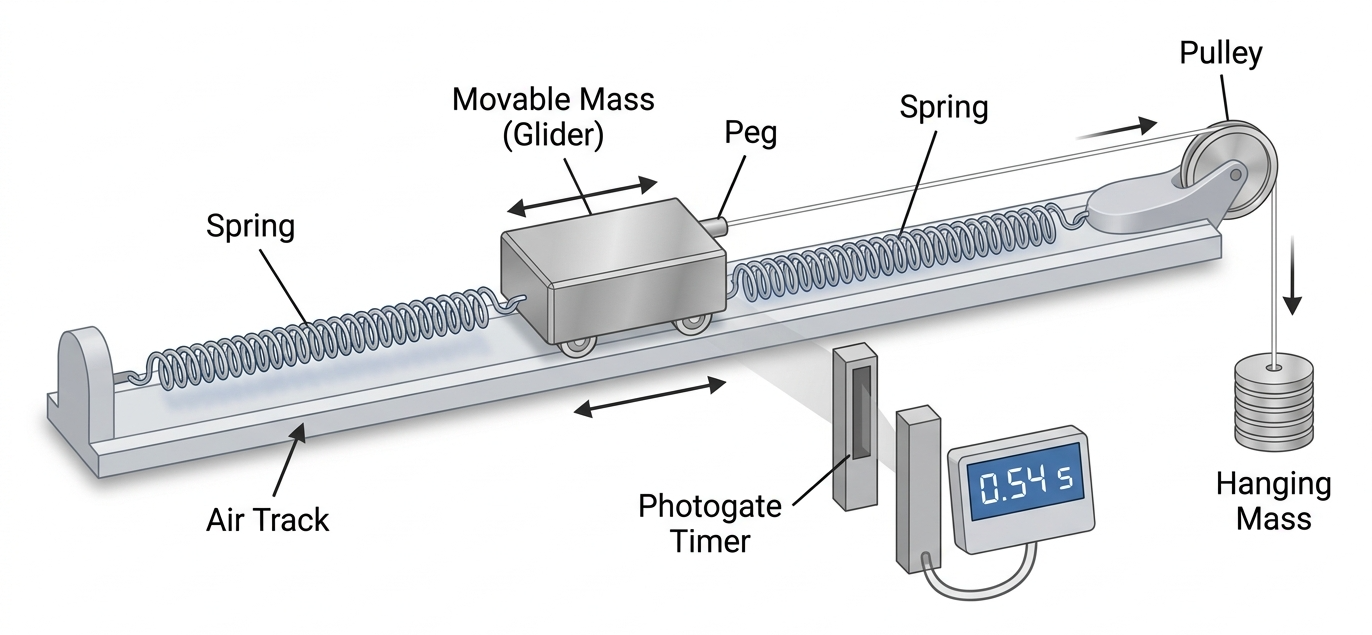
\includegraphics[width=12cm]{Mass_Spring_Apparatus.png}}
\end{center}

\textbf{Figure 1. Diagram of General Mass-Spring System Apparatus.}
Key components include airtrack with ruler, main gliding mass, additional masses, springs, pulley, variety of hanging masses, photogate timer. Figure is generated using the AI figure-making tool FigureLabs (2). 
\end{figure}
To measure the spring constant, a hanging mass is added to the platform and suspended from a pulley, exerting a force that causes the mass to displace. The hanging mass value is recorded and the force exerted is calculated (assuming force due to gravity is mass times gravitational acceleration) using the local gravity constant that is published for Pittsburgh: 9.80118 meters per second (1). The displacement from the equilibrium position is measured once the mass comes to rest. The accepted displacement uncertainty is based on the resolution of the meter stick that is to the nearest millimeter. Hanging mass and displacement measurements are repeated for the each spring configuration.

To find the empirical period for each system, we use the PASCO model ME-9215A calibrated photogate timer. We accept the uncertainty due to the timer's resolution of 0.1 milliseconds. We position the laser over the glider so that the glider edge passes through it three times each period. The timer is reset and the glider is pulled back a few centimeters before being released; the stopwatch stops when the period is complete. 10 period measurements are taken for each system; the system's measured period is the average of the 10 measurements and its uncertainty is calculated based on the distribution of measured values. 

To find the spring constant of the two spring configurations, force is plotted as a function of displacement according to equation 1. Then, assuming equation 3 for the predicted period and using the spring constant and total gliding mass values for each system, predicted period is plotted as a function of the average measured period for each system.

\section{Results and Discussion}
The spring constants of the two spring configurations are derived from the slope of the linear least-squares line of figures 2 and 3, where force is plotted with respect to displacement in accordance with equation 1. The spring constant of the 3 spring configuration is 17.15 $\pm$0.43 Newtons per meter with a reduced $\chi^2$ statistic of 0.59; the spring constant of the 4 spring configuration is 10.90 $\pm$0.17 Newtons per meter with a reduced $\chi^2$ statistic of 0.01. As expected, the system with only one spring on one end has greater resistance to stretching or compression.
\begin{figure}[H]
    \begin{adjustwidth}{-1in}{-1in}
        \centering
            \begin{subfigure}[b]{0.68\textwidth}
                
                \fbox{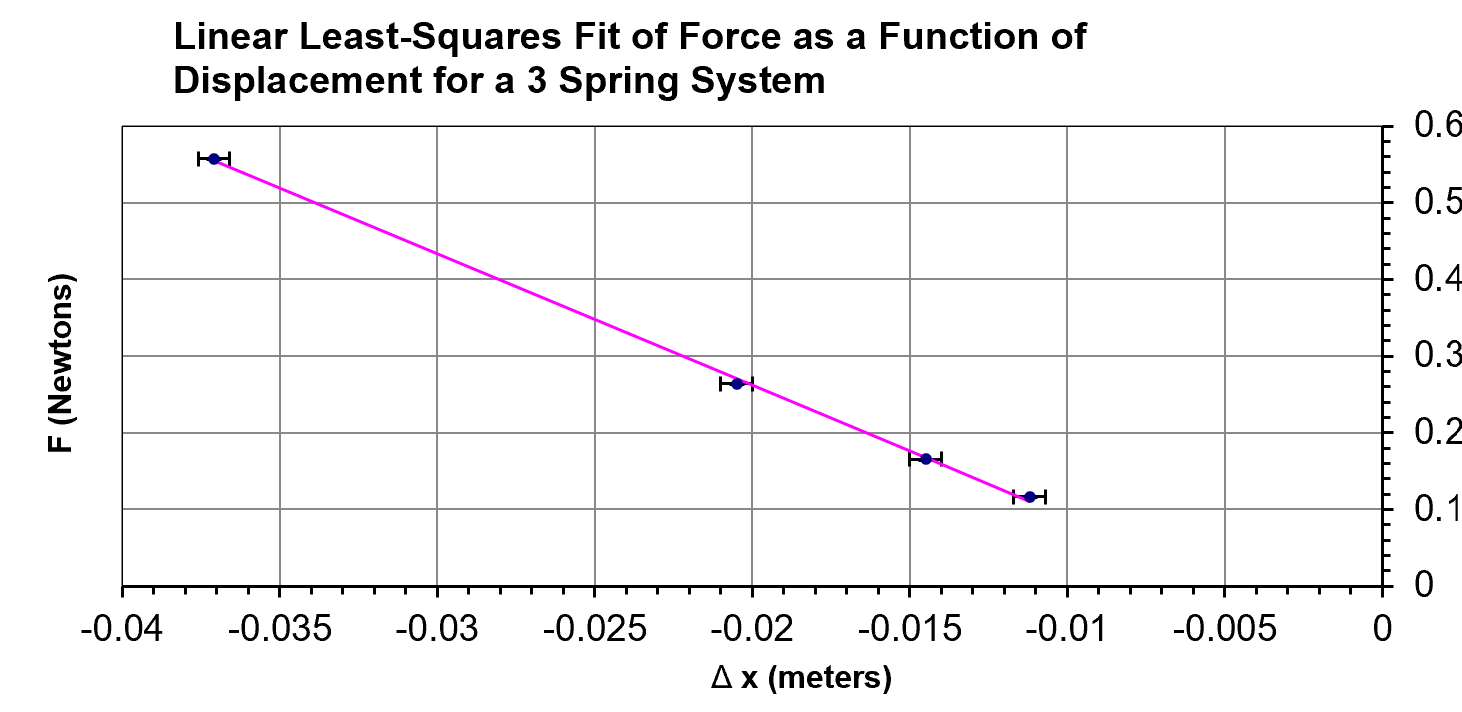
\includegraphics[width=\textwidth]{3_Spring_Constant_Figure.png}}
                \textbf{Figure 2. Force as a Function of Displacement for a 3 Spring System.}
                The equation for the linear-least squares fit line is y = -17.15 $\pm$0.43 - 0.0815 $\pm$0.0099. The negative of this value is the spring constant for a 3 spring system, independent of mass.

                
            \end{subfigure}%
            \hfill %
            \begin{subfigure}[b]{0.68\textwidth}
                \fbox{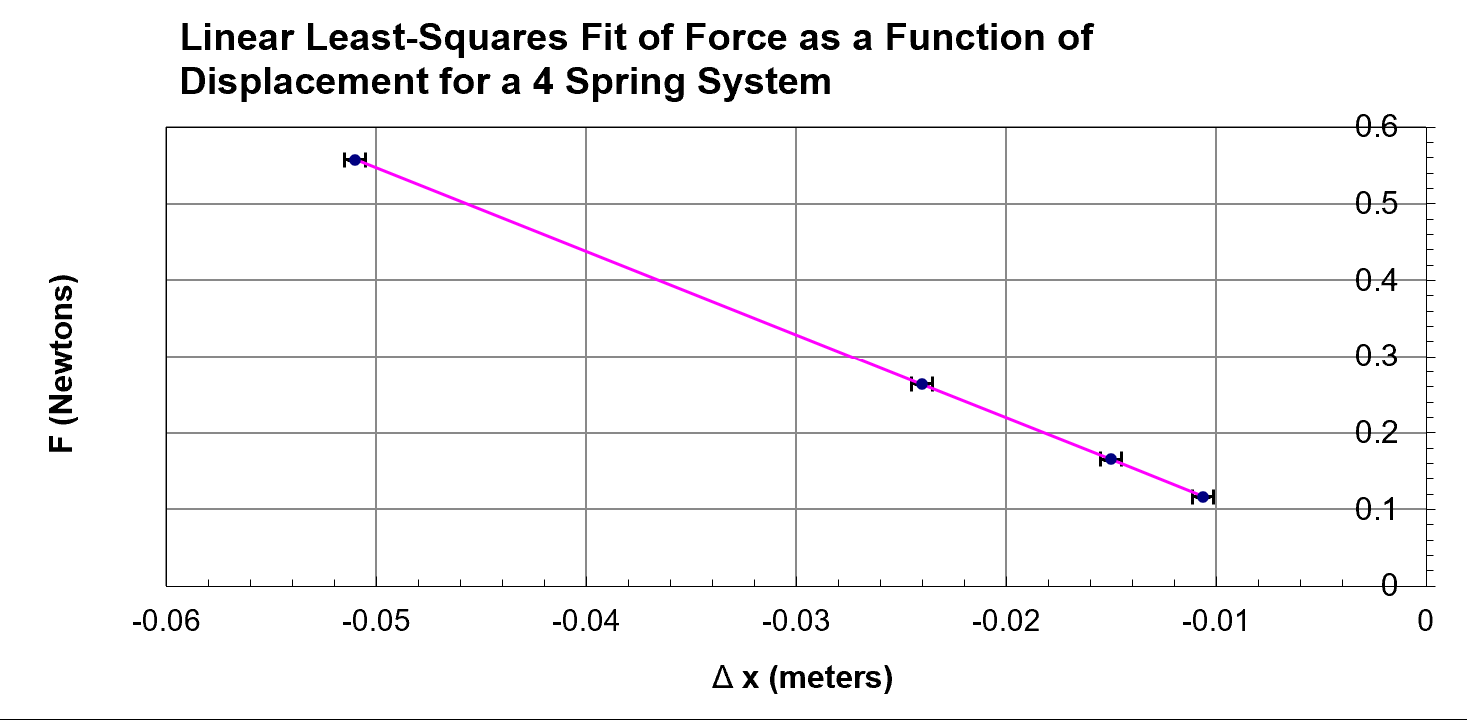
\includegraphics[width=\textwidth]{4_Spring_Constant_Figure.png}}
                \textbf{Figure 3. Force as a Function of Displacement for a 4 Spring System.}
                The equation for the linear-least squares fit line is y = -10.90 $\pm$0.17 + 0.0014 $\pm$0.0052. The negative of this value is the spring constant for a 3 spring system, independent of mass.
            \end{subfigure}

    \end{adjustwidth}
    
\end{figure}

The spring constants derived from the above linear least-square fit lines, along with the total mass measurements of each system, are used to calculate the predicted period using equation 3. The linear least-squares fit line for the predicted versus measured period in figure 4 has a slope of 1.017 $\pm$0.025 with a reduced $\chi^2$ statistic of 0.74. The standardized sigma divided by delta error for the slope is 0.69.

\begin{figure}[H]
    \fbox{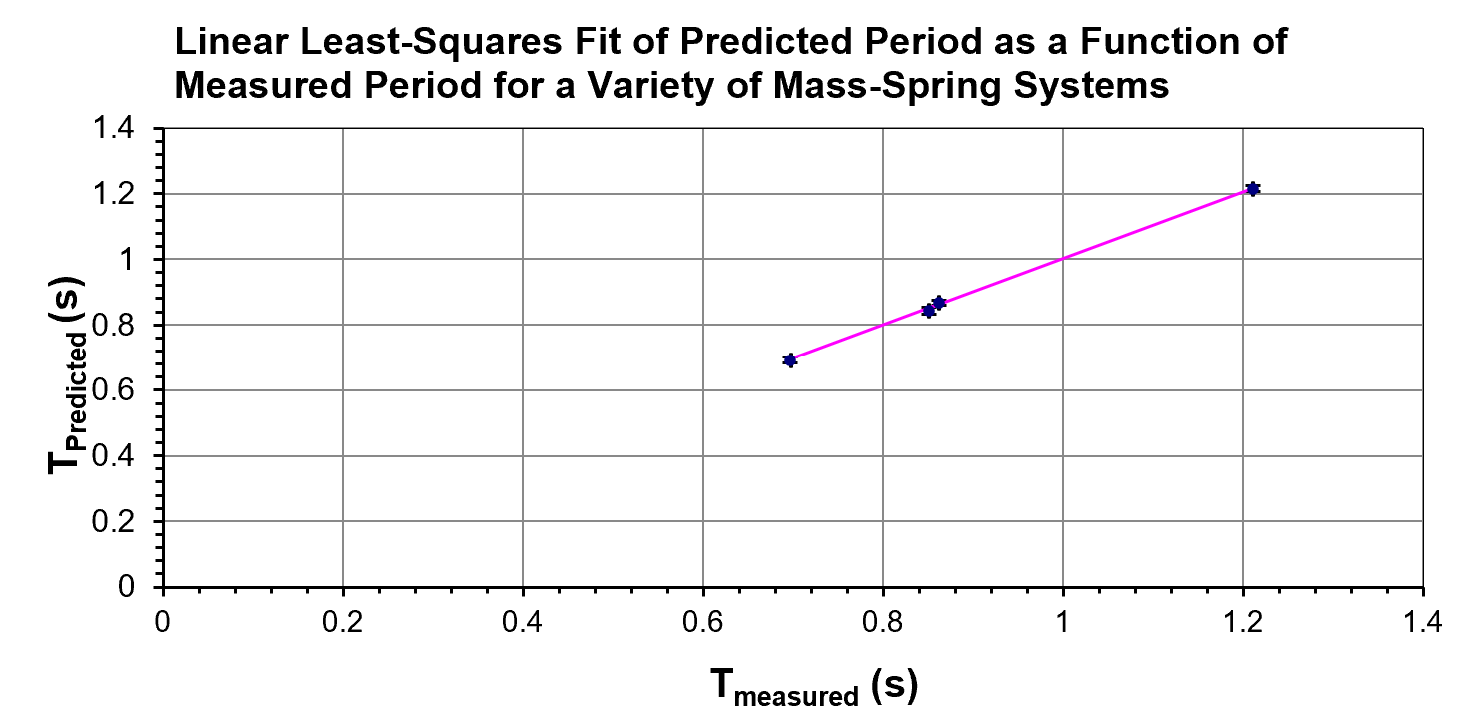
\includegraphics[width=12cm]{Comparison_Figure.png}}
    \textbf{Figure 4. Predicted Period as a Function of Measured Period.}
    The linear-least squares model equation is y = 1.017 $\pm$ 0.025 + 0.014 $\pm$ 0.022.
\end{figure}
The reduced $\chi^2$ statistic for figure 4 data is less than but close to 1, meaning the model is a good fit, but the error values may be overestimated. Thus, we can assume a linear relationship between expected and theoretical period.
The difference between the slope of the line in figure 1 and a slope of 1 is 0.69 standard deviations away from the expected difference of zero. This means that there is more than a 32 percent chance of getting a difference that is equal to or more extreme than it. Since this percentage means the difference is within 1 standard deviation from there being no difference, the measured and predicted period values are in good agreement. 

\begin{table}[H]
\begin{adjustwidth}{-1in}{-1in}
    \textbf{Table 1. Summary of Data for each System.} Standard error propagation is used to calculate accumulated error. 
    \begin{center}
        \makebox[1.2\textwidth][c]{%
        \begin{tabular}{|c|c|c|c|c|c|}
            \hline
             \textbf{System} &  \textbf{Mass $\mathbf{\pm\sigma_{m}}$ (g)} & \textbf{k $\mathbf{\pm\sigma_{k}}$ (N/m)} & \textbf{$\mathbf{T_{pred} \pm\sigma_{T_{pred}}}$ (s)} & \textbf{$\mathbf{T_{meas} \pm\sigma_{T_{meas}}}$ (s)} & \textbf{$\mathbf{\frac{\Delta}{\sigma_{\Delta}}}$}\\
             \hline
             3 Springs, no added mass & 207.990 $\pm$0.050 & 17.20 $\pm$ 0.43 & 0.6919 $\pm$ 0.0087 & 0.69678 $\pm$ 0.00010 & 0.558 \\
             
             4 Springs, no added mass & 207.990 $\pm$ 0.050 & 10.90 $\pm$ 0.17 & 0.8679 $\pm$ 0.0069 & 0.86178 $\pm$ 0.00020 & 0.889 \\
             3 Springs, 2 added masses & 308.210 $\pm$ 0.050 & 17.20 $\pm$ 0.43 & 0.842 $\pm$ 0.012 & 0.850840 $\pm$ 0.000062 & 0.808 \\

             4 Springs, 4 added masses & 408.010 $\pm$ 0.050 & 10.90 $\pm$ 0.17 & 1.2156 $\pm$ 0.0097 & 1.21100 $\pm$ 0.00027 & 0.478\\
            \hline
        \end{tabular}%
        }
    \end{center}
    
        
\end{adjustwidth}
\end{table}
The most relevant results of each mass-spring system are summarized in Table 1. The standardized errors for the difference in period values for each individual system are included. The standardized error values are all less than one indicating good agreement between measured and theoretical period for individual data points, in addition to overall agreement across data points. 

\section{Conclusion}
Our results demonstrate that the theoretical equation 3 for determining the period of oscillation for a free harmonic oscillator is valid and equivalent to the measured period, as there is no statistically significant difference between the predicted and measured period. Not only have we validated the theoretical equation, but also confirmed that we used valid experimental techniques to find the spring constant that the predicted period depended on.


\section{References}
1 Young and Freedman, University Physics, 14th Ed. Addison Wesley (2016) p. 418 \\
2 FigureLabs
\end{document}
